\documentclass{beamer}
\usepackage{multicol}
\usetheme{Copenhagen}

\title[Implementació d'un sistema criptogràfic per l'enviament del consum en sistemes de comptadors intel·ligents]{\textbf{Implementació d'un sistema criptogràfic per l'enviament del consum en sistemes de comptadors intel·ligents}}
\author{Oriol Alàs Cercós}

\institute[Universitat de Lleida]{
	\normalsize Francesc Sebé\\
	\texttt{francesc.sebe@udl.cat} \newline\newline
	Criptografia i Grafs\\
	Universitat de Lleida
}
\date{15 de juliol del 2021}

\bibliography{document}

\begin{document}
\begin{frame}
\centering

\Large\textbf{Implementació d'un sistema criptogràfic per l'enviament del consum en sistemes de comptadors intel·ligents}
\vspace{0.5cm}\\

\normalsize
Oriol Alàs Cercós
\\
\texttt{oriol.alas@udl.cat}
\vspace{0.5cm}\\
Francesc Sebé Feixas
\\
\texttt{francesc.sebe@udl.cat}
\small \vspace{0.3cm}\\
Criptografia i Grafs
\\
Universitat de Lleida
\vspace{0.5cm}\\
15 de juliol del 2021
\end{frame}
\begin{frame}
	\frametitle{Taula de continguts}
	    \begin{columns}[onlytextwidth,T]
		\begin{column}{.45\textwidth}
			\tableofcontents[sections=1-2]
		\end{column}
		\begin{column}{.45\textwidth}
			\tableofcontents[sections=3-5]
		\end{column}
	\end{columns}
\end{frame}

\section{Introducció}
\subsection{Plantejament}
\begin{frame}{Introducció}
	\begin{figure}
		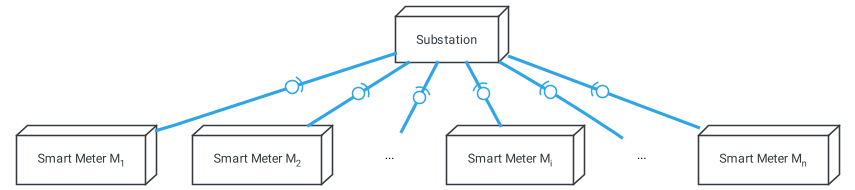
\includegraphics[width=10cm]{../umls/network.png}
	\end{figure}
\end{frame}
\subsection{Objectius}
\begin{frame}{Introducció}{Objectius}
	Objectius:
	\begin{itemize}
		\item Estudiar la solució proposada.
		\item Posar en context el xifratge homomòrfic i el criptosistema asimètric ElGamal.
		\item Implementar un client que simuli un comptador intel·ligent.
		\item Implementar un servidor que simuli una subestació d'una comunitat de comptadors.
		\item Realitzar un estudi dels costs del protocol.
	\end{itemize}
\end{frame}

\subsection{Xifratge simètric i asimètric}

\subsection{Xifratge homomòrfic}

\section{Propostes}
\subsection{Tipus de propostes}
\begin{frame}
	\frametitle{Tipus de propostes}
	\begin{itemize}
		\item \alert<1-2>{Propostes pertorbatives}\\
		\only<2>{
			\vspace{1em}
			Afegir un soroll a les lectures per tal de
transmetre un resultat diferencial.
			\[\sum_{i=1}^{N} m_i \approx \sum_{i=1}^{N} (m_i + x_i)\]}
		\item \uncover<3->{\alert<3-4>{Propostes anònimes}}
		\only<4>{
			\begin{block}{Funcionament}
				Anonimitzar les dades del consum per tal de no poder determinar fàcilment una llar.
			\end{block}
			\begin{itemize}
				\item High-Frequency ID
				\item Low-Frequency ID
			\end{itemize}
		}
		\item \uncover<5->{\alert<5->{Propostes agregatives}}\\
		\only<6>{
			\vspace{1em}
			Els comptadors s’agreguen en comunitats per tal de sumar les seves
lectures abans de transmetre-les a la subestació.
			\vspace{0.5em}
			\begin{itemize}
				\item Distribuïdor de claus.
				\item Xifratge homomòrfic.
			\end{itemize}
		}
	\end{itemize}
\end{frame}

\subsection{Proposta de }
\begin{frame}
	\cite{busom}
\end{frame}
\subsection{L'actual proposta}

\begin{frame}{Equation}
	\begin{block}{Equation without numbers} 
		\begin{equation*}
			J(\theta) = \mathbb{E}_{\pi_\theta}[G_t] = \sum_{s\in\mathcal{S}} d^\pi (s)V^\pi(s)=\sum_{s\in\mathcal{S}} d^\pi(s)\sum_{a\in\mathcal{A}}\pi_\theta(a|s)Q^\pi(s,a)
		\end{equation*}
	\end{block}
	%    \begin{exampleblock}{Multiple equations\footnote{If containing text in equations,use $\backslash$mathrm\{\} or $\backslash$text\{\}}}
	%       
	%        \begin{align}
	%            Q_\mathrm{target}&=r+\gamma Q^\pi(s^\prime, \pi_\theta(s^\prime)+\epsilon)\\
	%            \epsilon&\sim\mathrm{clip}(\mathcal{N}(0, \sigma), -c, c)\nonumber
	%        \end{align}
	%    \end{exampleblock}
\end{frame}

\begin{frame}
	\begin{block}{Equation with numbers}
		% Taken from Mathmode.tex
		\begin{multline}
			A=\lim_{n\rightarrow\infty}\Delta x\left(a^{2}+\left(a^{2}+2a\Delta x+\left(\Delta x\right)^{2}\right)\right.\label{eq:reset}\\
			+\left(a^{2}+2\cdot2a\Delta x+2^{2}\left(\Delta x\right)^{2}\right)\\
			+\left(a^{2}+2\cdot3a\Delta x+3^{2}\left(\Delta x\right)^{2}\right)\\
			+\ldots\\
			\left.+\left(a^{2}+2\cdot(n-1)a\Delta x+(n-1)^{2}\left(\Delta x\right)^{2}\right)\right)\\
			=\frac{1}{3}\left(b^{3}-a^{3}\right)
		\end{multline}
	\end{block}
\end{frame}


%\begin{frame}[fragile]{\LaTeX{} Commands}
%    \begin{exampleblock}{Commands}
%        \centering
%        \footnotesize
%        \begin{tabular}{llll}
%            \cmd{chapter} & \cmd{section} & \cmd{subsection} & \cmd{paragraph} \\
%            Chapter & Section & Subsection & Paragraph \\\hline
%            \cmd{centering} & \cmd{emph} & \cmd{verb} & \cmd{url} \\
%            Centre Align & Emphasis & Verbatim & Hyperlink \\\hline
%            \cmd{footnote} & \cmd{item} & \cmd{caption} & \cmd{includegraphics} \\
%            Foodnote & Item & Caption & FigP\&Pic \\\hline
%            \cmd{label} & \cmd{cite} & \cmd{ref} \\
%            Label & Citing & Referring\\\hline
%        \end{tabular}
%    \end{exampleblock}
%    \begin{exampleblock}{Environment Command}
%        \centering
%        \footnotesize
%        \begin{tabular}{lll}
%            \env{table} & \env{figure} & \env{equation}\\
%            Table & Figure & Equation \\\hline
%            \env{itemize} & \env{enumerate} & \env{description}\\
%            Bullets & Numbering & Description \\\hline
%        \end{tabular}
%    \end{exampleblock}
%\end{frame}



\begin{frame}{Tables}
	\begin{table}[hbt]
		\begin{tabular}{l|cc}
			1& 2& \\
			\hline
			3& 4& \\
			5& 6&
		\end{tabular}
		\caption{}
	\end{table}
	
\end{frame}

%% ---------------------------------------------------------------------------
% This frame show an example to insert multi-columns
%\begin{frame}{Multi-columns}
%    \begin{columns}{}
%        \begin{column}{0.5\textwidth}
%            \justify
%            É possível colocar mais de uma coluna utilizando os comandos de $\backslash$begin\{column\}\{\} e $\backslash$end\{column\}
%        \end{column}
%        \begin{column}{0.5\textwidth}
%            \justify
%            Porém, o espaçamento deve ser proporcional entre as colunas para que estas colunas não entrem em coflito. O espaçamento é dado pelo segundo argumento do $\backslash$begin.
%        \end{column}
%    \end{columns}
%    \begin{columns}{}
%        \begin{column}{0.5\textwidth}
%            \justify
%            É possível colocar mais de uma coluna utilizando os comandos de $\backslash$begin\{column\}\{\} e $\backslash$end\{column\}
%        \end{column}
%        \begin{column}{0.5\textwidth}
%            \justify
%            Porém, o espaçamento deve ser proporcional entre as colunas para que estas colunas não entrem em coflito. O espaçamento é dado pelo segundo argumento do $\backslash$begin.
%        \end{column}
%    \end{columns}     
%\end{frame}


%% ---------------------------------------------------------------------------
% Reference frames
%\begin{frame}[allowframebreaks]
%    \frametitle{Reference}
%    \printbibliography
%\end{frame}

%% ---------------------------------------------------------------------------
% Final frame
\section{Disseny de la implementació}
\subsection{Datagrames}
\subsection{Criptografia}
\subsection{Patró Màquina-Estat}
\section{Anàlisi de costos}
\subsection{Logaritme discret}
\subsection{Comparació de propostes}
\begin{frame}[allowframebreaks]
	\bibliography{references.bib}
\end{frame}
\end{document}